\subsection{Power Supply and Voltage Regulation}
\noindent Each component of the FORWARD walker requires a specific amount of voltage. In order to cater to each of these needs, we will first need to have separate power supplies. The motors driving the wheels as well as the headlight both demand 12V, so they will require a larger power supply that only outputs 12V. The remainder of the components, contrarily, all use a much smaller power supply. Thus, we will utilize a large power supply and a small power supply (both of which are rechargeable).\\

\noindent For the smaller power supply, we will need to employ voltage regulation to provide the correct amount of voltage between the different units. The microcontroller and accompanying sensors all require one voltage supplied to the MCU and distributed to the sensors. The ESP32 is rated as a 3.3V device\cite{sparkfun12024} and powers the sensors using the GPIO pins. However, the haptic motors require a separate power supply from the MCU as they are operated using a motor driver rated for 5V. The camera module is also powered separately from the MCU with a supply of 5V. The ultrasonic sensors also perform better at a rated voltage of 5V. In order to deliver enough voltage for both the MCU, the camera module, the ultrasonics, and the haptic motors, we will use a 5V battery pack (originally designed to charge phones) and from there add voltage regulation circuits to the PCB. The haptic motors and the camera module will accept the simple output of the battery pack at 5V, however, the MCU, LiDAR, and MCU will need this voltage to be stepped down 3.3V. This circuit will be implemented within the PCB.

\subsection{Avoidance Subsystem}
\noindent This subsystem is dedicated to the movement of the walker as pertains to the motors and mechanics. FORWARD has a prescribed method of steering and braking that will be expanded upon. There have also been changes to the design throughout the project affecting our choice and application of the motors to be discussed.
% intro paragraph

\subsubsection{Motor Control System}
\noindent In order for the motors to rotate, they must be controlled by a control system. Once the user initiates FORWARD by powering it on, there will be a dial (potentiometer) that the user has can spin in order to select the starting speed. This dial will have divots or braille for the user to feel to determine if they are selecting a slower or faster speed. This constant will then be sent by the potentiometer to the MCU (controller), which will process the input and send commands to the motor driver. The motor driver will receive the commands from the MCU and apply the correct voltage and PWM signal to the motors, which are the actuators performing the action of spinning the wheels. As the walker drives forward, the sensors will be continually reading data and providing feedback to the MCU. When an obstacle is encountered, the MCU transmits new commands to the motor driver in accordance with the sensors and camera. The motor driver will then alter the PWM signal and the motors will change direction or apply brakes accordingly.\\

\noindent The other components of feedback operate in a similar closed loop. The haptic motors use the same diagram, except their speed is not dependent on the potentiometer and only activate when an obstacle is detected by the sensors and camera. In addition, the output of the haptic motors is vibration instead of motion. The audio feedback follows a similar process, however, it is ideally controlled directly by the MCU (although may have need of another circuit to act as a driver) and the output is playing back audio files of the objects detected by the camera.

\begin{figure}[H]
	\centering
	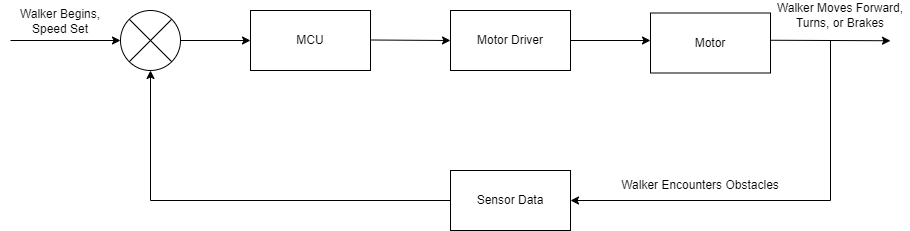
\includegraphics[width=1\textwidth]{./Images/control_system_speed}
	\caption{\label{fig:Motor_Control_System}Motor Control System Diagram}
\end{figure}

% do we fix the wheels in place? most of them swivel like castors - that's fine, rear-wheel drive.
\subsubsection{Wheel Rotational Motion}
\noindent The rollator wheels will dictate the way by which turning can be achieved. There are four wheels. We call the distance in between the front wheels $axel_f$ and the distance in between the rear wheels $axel_r$. Upon initial inspection of the rollator once acquired, we see that $axel_f > axel_r$.
%The measurements of the wheels are included in figure \ref{rollator-amaz}.

\noindent From a top view, the rear two wheels can be viewed as simple points. They do not swivel, and thus can rotate in place but cannot do horizontal translation, stipulated by friction and attachment to the rollator frame. Of course, they can also roll and move forward.\\

\noindent In addition, the front wheels are on a $360^{\circ}$ swivel. They can also be modeled as points in a sense; however, their orientation changes.\\

\begin{figure}[H]
	\centering
	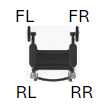
\includegraphics[width=.25\textwidth]{./Images/wheel_assignment.png}
	\caption{\label{fig:Wheel_assignment}Wheel Assignment}
\end{figure}

\noindent \underline{\textit{Case 1}} (extreme): Both wheels rotate. The front wheels translate.\\

\begin{figure}[H]
	\centering
	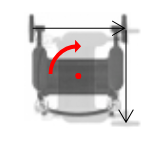
\includegraphics[width=.25\textwidth]{./Images/case1.png}
	\caption{\label{fig:case-one}Case 1: Rotation (not ideal due to friction)}
\end{figure}

\noindent \underline{\textit{Case 2}} (extreme): one wheel rotates, the other stationary. The front wheels revolve.\\

\begin{figure}[H]
	\centering
	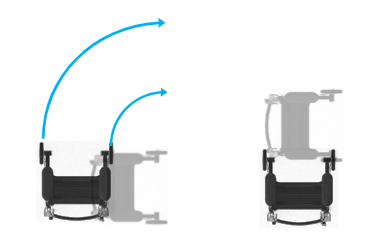
\includegraphics[width=.5\textwidth]{./Images/case2.png}
	\caption{\label{fig:case-two}Case 2: Stationary motor, rotating motor}
\end{figure}

\noindent \underline{\textit{Case 3}} Veering. motor speeds may not have to change. User can veer based on feedback, and gentle guidance provided by FORWARD.\\

\begin{figure}[H]
	\centering
	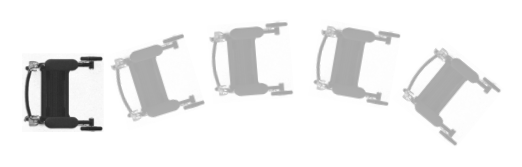
\includegraphics[width=.5\textwidth]{./Images/case3.png}
	\caption{\label{fig:case-three}Case 3: Veering}
\end{figure}

% talking more about one wheel motor faster than the other. fusing user steering with FORWARD guidance.\
\subsubsection{Turning Mechanics}
\noindent A major question pertaining to obstacle avoidance is our mechanism of steering. As mentioned previously in section 3.2.7, we wish to rely solely on the DC motors for steering control in order to minimize mechanical complexity.  To refresh, rather than using a servo motor or other apparatus to turn an axle that steers the wheels, we will use two separately controlled DC motors with no axle. Because each of these motors are controlled independently, each will assume a different speed in order to steer the wheels, else remain at equal speeds to move forward in a straight line. The angle of the turn is determined by the drop in speed of the motor adjacent to the turning direction. As an example, if the walker needs to veer very sharply to the left, the left motor will either halt rotating or rotate very slowly compared to the right motor. On the contrary, if simply a slight turn is needed to avoid an obstacle, both motors will drive at comparable speeds with one motor slightly decreased in speed. One potential issue with this strategy is that FORWARD can only move in a straight line if both motors are rotating at exactly the same speed; otherwise, the walker may drift toward one side or the other, as opposed to an axle that is driving the wheels symmetrically. However, we are using identical motors from the same manufacturer and applying the same amount of voltage. It is possible that there will still be some amount of drift due to manufacturing errors, wire resistance, or other unknown factors. Nonetheless, we do not anticipate drift to be much of an issue as the walker can also correct itself upon straying from the path, as it will detect an obstacle, whether the obstacle is a curb, the grass, the road, etc.

% what methods and considerations do we have when sticking the motors on the rollator?
\subsubsection{Motor Installation}
% reconciling measurements acquired of the wheel diameter, weight, etc, with the torque of the DC motors.
\noindent \underline{\textit{Calibration}}\\
\noindent Our initial selection for DC motors driving the wheels were the S55B-150 motors from Chapter 3. However, there were several factors that we did not account for in purchasing these motors. To begin with, these motors are brushless three-phase DC motors. After discussing with Dr. Weeks, one of our coordinators for Senior Design, we learned that in order to program these motors to function properly, each of the phases needs to be aligned within the programming. This would be a very difficult process, especially considering that there is hardly any documentation given for the S55B-150 given by the seller. In considering this advice, we purchased instead \cite{amazon12024}. Although these motors are only 40-50W, they nonetheless provide plenty of torque to drive the walker due to the gearbox increasing torque. We will eventually need to test the speed of the walker to see if it will be able to achieve one of our requirements of 6mph. The motors with no load can rotate up to 30,000rpm, which with 8" diameter wheels translates to over 700mph \cite{lucidar2024}. However, this number will drastically change as up to 60lbs plus the weight of the user's body leaning against the walker acts as a large load. We will simply need to test the speed of the walker in Senior Design II and keep in mind that speed may not be a requirement that is met.\\

% does simply glueing the haptic motors on the handlebar underside sufficiently vibrate the handlebars to where the user notices? how much power would that require?
\noindent \underline{\textit{Vibrating Handlebars via Haptics}} -  Our design for haptic feedback includes small ERM motors that will spin at a rapid rate with no load. Attached underneath the handlebars to the walker, the rapid spinning will cause a vibration noticeable to the user. This is a vital portion of guidance to the user, as our desire with this project is to provide a solution for people with a broad range of sensory disorders. If the user has issues with using the audio feedback or is unable to hear, the haptic motors provide similar directions describing the surroundings and motion of the walker. When our FORWARD walker detects and identifies obstacles, the user must be aware that an obstacle has been detected, what the obstacle or danger level is, and what steps the walker will take in order to avoid the obstacle. Otherwise, the user may act contrary to the walker or stumble in response to the sudden change in movement. For example, if FORWARD approaches a wall and comes to a stop, the user, who is walking with the walker, could run into the walker or be lunged forward by inertia apart from feedback. The haptic motors are being controlled by a motor driver communicating with the ESP32. This motor driver receives commands from the ESP32, which also combines input from the various sensors, and sends commands to the motors that vibrate accordingly.

% talk about how the rollator has pneumatic handle squeeze brakes but braking can also be achieved by locking the DC motors
\subsubsection{Emergency Braking}
\noindent FORWARD of necessity must also be able to respond to obstacles by braking. The chassis we have chosen to use already contains a manual braking system. There are pneumatic triggers beneath the handlebars that apply the brakes upon compression. We would like to preserve these manual brakes for the sake of safety in case any electrical or software issues arise. However, we also need FORWARD to brake automatically in response to obstacles. We will accomplish this by programming the motors to first slow down their speed to a stop and then reverse the direction of the motors until the entire walker is no longer in motion. This is known as dynamic braking\cite{electricaleasy2014}. We will need to test the braking to determine the correct timing of when the walker comes to a complete stop so that we know when to stop the motors after reversing. If we are unable to correctly time the motors, we may need a way to sense when the walker has come to a complete halt. This may be possible using the camera or a motion sensor \cite{bayalarm2024}.

%issue about user trying to steer when they shouldn't
\subsubsection{Reconciling User Control and Automatic Guidance}
\noindent There is also an issue of user error that must be considered. Our design is intended for the walker to lead the user, not for the user to lead the walker. This is not much of an issue with braking as there should not be any safety issues in the user applying manual brakes when not needed. Although this may wear down the motors over time as the rotor is prevented from rotating, we do not foresee any major consequences. However, the user may try to steer the walker in the wrong direction when not directed by the walker. This could cause a serious issue in the safety of the user if they steer the walker into an obstacle. Currently, if the user tried to steer the walker, the walker would automatically correct itself upon encountering an obstacle and warn the user of the obstacle. A more advanced solution could be pressure sensors that detect the body weight of the user and can sense if the user is leaning a particular way. However, this is outside the scope of our project, although in production this issue would certainly need to be addressed.\\

\subsubsection{Physical Object Avoidance Margins}
\noindent One of the main criteria for FORWARD is that it must avoid obstacles, and here we address the distance of the obstacles from the user before the rollator turns or brakes. If the obstacle is right in front of the user, one of our requirements is that the walker must be able to come to a complete stop within one second. If FORWARD is propelling at the maximum speed of 6mph, it can cover up to 8.8 feet in one second. However, this does not account for the acceleration as the walker slows down. It is also unlikely that this maximum speed will be used in practice at it is the average running speed of a human. We can set different distance ranges per potentiometer reading that sets the speed. So, if an obstacle is detected within x(v) feet in front of FORWARD, where the distance x is a function of the velocity v, then the walker will halt for the obstacle. The most likely speed to be selected is 2mph, as this is the average walking speed for a human, which will correspond to braking for obstacles in a 3 foot distance.\\

\noindent Calculations must also be made for the angle and distance at which the walker must turn to avoid obstacles. Objects in the way of the walker will still be detected within the same range as stated above, however, the response of FORWARD will differ if the object can be avoided by steering to the right or to the left. If the right ultrasonic sensors detect an object within x(v) feet of the walker and comparisons with the camera data (detecting the location of the obstacle within the frame) indicate that the walker must veer left, then the wheels will be adjusted in response. The angle at which the rollator will turn away from the obstacle is dependent on the motion and location of the obstacle. If, for example, a tree stood in the path of the user, the MCU will calculate using the camera frame the location that FORWARD will be next to the tree plus a clearance of 6". If the tree is directly ahead, for example, then the distance calculated will be half of the width of the tree + the width of the walker + 6" clearance. Then calculating the angle at which FORWARD must veer is a matter of simple trigonometry.
\[ \theta = tan^{-1}(o/a)\]
\noindent where o = the distance between obstacle and future position of the walker and a = the distance from the walker to the obstacle.

\begin{figure}[H]
	\centering
	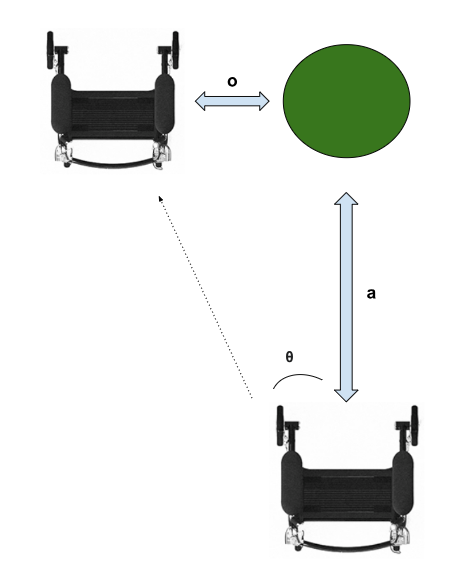
\includegraphics[width=.5\textwidth]{./Images/margin.png}
	\caption{\label{fig:margin}Veering Angle}
\end{figure}

%\noindent implementation of earpiece being available to user. obstacle classifications.\\
